% 自分用LaTeXテンプレート
% タイプセットはupLaTeX, dvipdfmxを使用,スタイルはjsarticle

\documentclass[uplatex, a4paper]{jsarticle}
\usepackage[dvipdfmx]{graphicx}

\usepackage{tabularx}   % 表
\usepackage{layout}     % レイアウト

% ---数式関係---
\usepackage{amsmath}    % ams math
\usepackage{bm}         % ボールド

\usepackage{url}    % URLを書くため

%\pagestyle{empty}  % ページ番号消去
\pagestyle{plain}   % ページ番号表示

% ---レイアウトパラメータ---
\usepackage[left=25mm,right=25mm,top=20mm,bottom=20mm, includefoot]{geometry}

\def\Vec#1{\mbox{\boldmath $#1$}}   % ベクトル(ボールド)の定義

\renewcommand{\tablename}{Table}    % 表番号フォーマットをTableへ
\renewcommand{\figurename}{Fig.}    % 図番号フォーマットをFig.へ

\renewcommand{\baselinestretch}{0.8}    % 行間の調整

\title{\Huge タイトル} 
\author{\huge 書いた人の名前}
\date{\today}

% ---ドキュメント開始---
\begin{document}

\maketitle  % タイトル生成

\section{テンプレート}
ここに本文を書く.これは自分用のテンプレートです.

\section{なんでupLaTeXなの?}
研究室での \LaTeX の形式がこれだったから

%input{Folder/documentname.tex} % ファイルをインポート

\subsection{使い方}
\begin{itemize}
    \item このテンプレートには各種設定や基本的なコマンドの使い方などが含まれます
    \item 不要な部分は削除してお使いください
    \item やる気がある限り順次更新されていくと思います
\end{itemize}

図はPDF形式で貼りましょう.図\ref{fig:sample}はサンプル画像です.

% 図を貼る
\begin{figure}[h]   % h: この場所に t: ページのトップに b: ページのボトムに p: 新しいページを作って画像を貼る
    \centering              % 中央揃え
    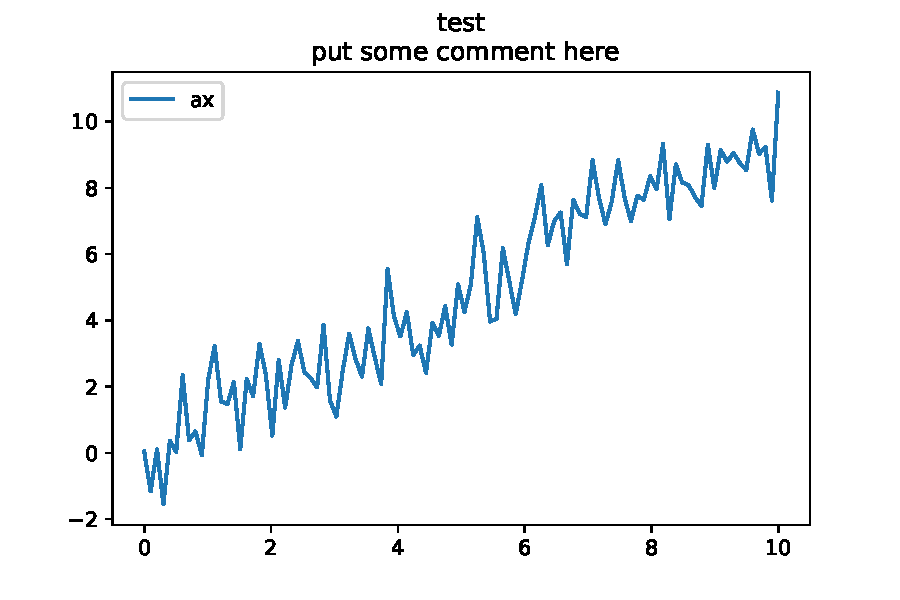
\includegraphics[width=60truemm,clip]{Images/graph_sample.pdf}
    \caption{Sample Picture}% 図のタイトル(英語)
    \label{fig:sample}      % 参照用ラベル
\end{figure}

% 横に並べて図を貼る(自動改行を防ぐためにtabularを使う)
\begin{figure}[h]
  \begin{center}    % 中央揃え
    \begin{tabular}{c}
      \begin{minipage}{.45\linewidth}   % 左側の図
      \centering
      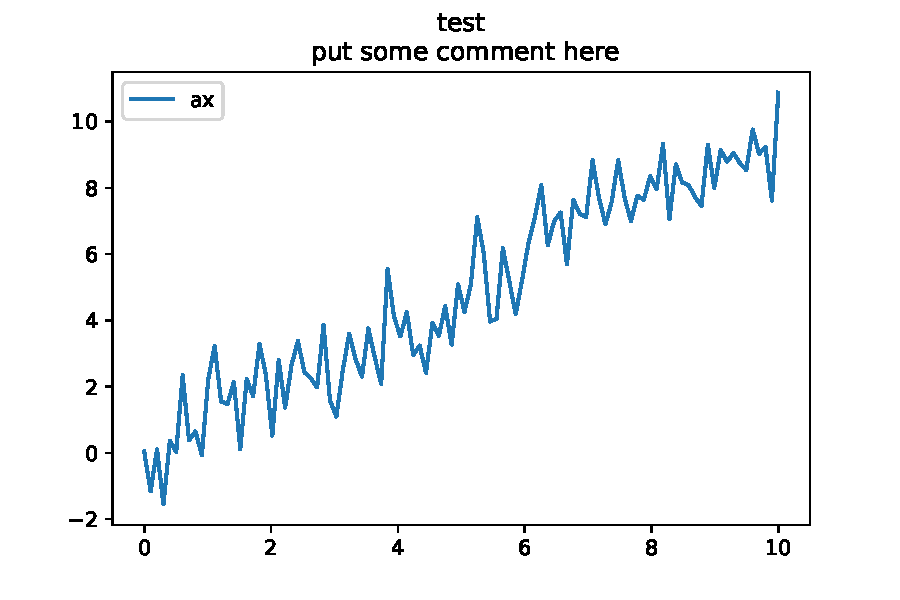
\includegraphics[width=60truemm,clip]{Images/graph_sample.pdf}
      \caption{Sample Picture(Left side)} % 図のタイトル(英語)
      \label{fig:sample_l}                % 参照用ラベル
      \end{minipage}
      
      \begin{minipage}{.45\linewidth}   % 右側の図
      \centering
      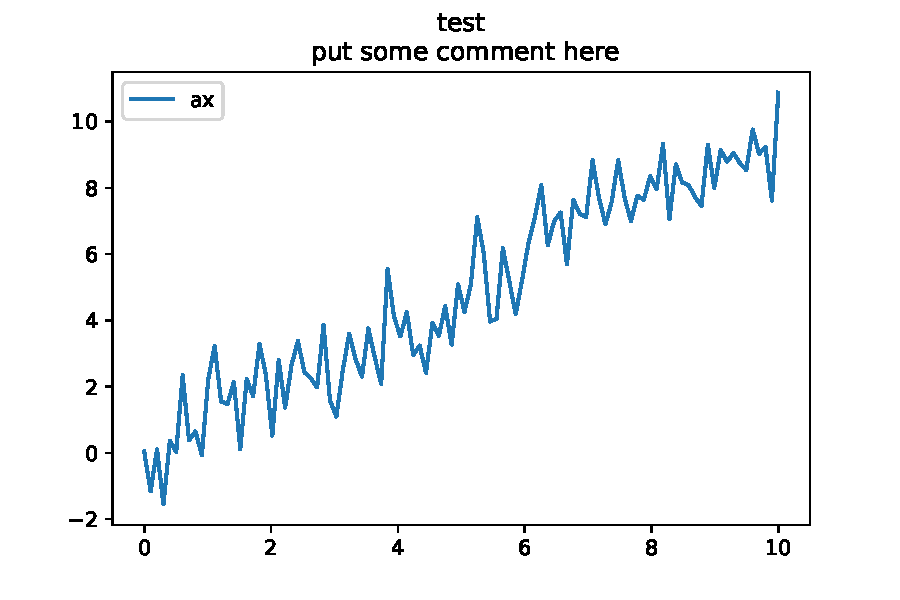
\includegraphics[width=60truemm,clip]{Images/graph_sample.pdf}
      \caption{Sample Picture(Right side)}% 図のタイトル(英語)
      \label{fig:sample_r}                % 参照用ラベル
      \end{minipage}
    \end{tabular}
  \end{center}
\end{figure}

\end{document}
% --- ドキュメント終了 ---
